\documentclass[11pt, letterpaper, conference, final, twocolumn]{ieeeconf}
\IEEEoverridecommandlockouts
\overrideIEEEmargins

% packages
\usepackage{amsmath, amsfonts, amssymb, bm, enumerate, url}%, flushend}
\usepackage[boxruled, vlined, linesnumbered]{algorithm2e}
\usepackage[usenames, dvipsnames]{color}
\usepackage[pdftex, xetex]{graphicx}
\usepackage[font={small}]{caption}
\usepackage{float, colortbl, tabularx, multirow, subfig, environ}
\usepackage{pgf, tikz}
\usetikzlibrary{arrows,automata}
\usepackage[normalem]{ulem}

\usepackage[bookmarks=true]{hyperref}
\hypersetup{
colorlinks=true, linkcolor=red, citecolor=blue, filecolor=magenta, urlcolor=blue
%linkcolor=black, citecolor=black, filecolor=black, urlcolor=black
}
\usepackage{url, cite}

% macros
\providecommand{\abs}[1]{\ensuremath \left| #1 \right|}
\providecommand{\norm}[1]{\ensuremath \lVert#1\rVert}
\providecommand{\given}{\, \vert \,}
\providecommand{\cal}[1]{\ensuremath \mathcal{#1}}
\providecommand{\qed}{\hfill \mbox{\raggedright \rule{0.1in}{0.1in} } }

\providecommand{\aeq}[1]{\begin{align} #1 \end{align}}
\providecommand{\aeqs}[1]{\begin{align*} #1 \end{align*}}
\providecommand{\beq}[1]{\begin{equation}#1\end{equation}}
\providecommand{\beqs}[1]{\begin{equation*}#1\end{equation*}}
\providecommand{\trm}[1]{\ensuremath \textrm{#1}}
\providecommand{\enum}[2]{\begin{enumerate}[#1]{#2}\end{enumerate}}
\providecommand{\ilist}[1]{\begin{itemize}{#1}\end{itemize}}
\providecommand{\ag}[1]{\ensuremath \left\langle#1\right\rangle}
\providecommand{\bee}{\begin{enumerate}}
\providecommand{\eee}{\end{enumerate}}
\providecommand{\bm}[1]{\begin{bmatrix}#1\end{bmatrix}}

\usepackage{theorem}
\newtheorem{theorem}{Theorem}
\newtheorem{proposition}[theorem]{Proposition}
\newtheorem{lemma}[theorem]{Lemma}
\newtheorem{corollary}[theorem]{Corollary}
\newtheorem{problem}[theorem]{Problem}
%\theoremstyle{definition}
\newtheorem{definition}[theorem]{Definition}
\newtheorem{example}[theorem]{Example}
\newtheorem{note}[theorem]{Note}
\newtheorem{remark}[theorem]{Remark}
%\theoremstyle{plain}
\newtheorem{assumption}[theorem]{Assumption}

\newcommand{\PP}{\ensuremath \mathbb{P}}
\newcommand{\EE}{\ensuremath \mathbb{E}}

% margins
\setlength{\marginparwidth}{0.6in}
\definecolor{darkgreen}{rgb}{0,0.6,0} \newcommand{\dg}{\color{darkgreen}}
\definecolor{fullred}{rgb}{0.85,.0,.1} \newcommand{\fr}{\color{fullred}}
\definecolor{darkblue}{rgb}{0,0,1.0} \newcommand{\db}{\color{darkblue}}
\definecolor{brown}{rgb}{0.54,.27,0} \newcommand{\br}{\color{brown}}

\newcommand{\pcm}[2]{{\dg #1}\marginpar{\tiny\noindent{\raggedright{\dg[PC]}\br{ #2} \par}}}
\newcommand{\vsm}[2]{{\fr #1}\marginpar{\tiny\noindent{\raggedright{\dg[VS]}\db{ #2} \par}}}
%\renewcommand{\margin}[2]{#1}
\newcommand{\ignore}[1]{}

% save space
\newcommand{\algsize}{\footnotesize}
\setlength{\floatsep}{0.05in}
\setlength{\textfloatsep}{0.1in}
\setlength{\intextsep}{0.05in}
\setlength{\belowcaptionskip}{0.01in}
\setlength{\abovecaptionskip}{0.1in}
\setlength{\abovedisplayskip}{0.08in}
\setlength{\belowdisplayskip}{0.08in}

\begin{document}
\title{\bf Twitter-based Mood Evaluation
	\thanks{$^*$Chemical Engingeering Department, MIT. Email: \href{mailto:vishnusr@mit.edu}{vishnusr@mit.edu}}
	\thanks{$^\dag$Laboratory of Information and Decision Systems, MIT. Email: \href{mailto:pratikac@mit.edu}{pratikac@mit.edu}}
	\thanks{Note: Equal contribution from both authors}
}
\author{Vishnu Sresht$^*$ \qquad Pratik Chaudhari$^\dag$}
\maketitle

\begin{abstract}
By providing a convenient, readily-accessible way to reach out to a global audience, twitter has revolutionized the way we broadcast our feelings to the rest of the world. In addition to its empowerment of the diva within us all, Twitter's meteoric rise in popularity has enabled every one of us to listen to the voices of millions and comprehend mankind's \textit{zeitgest} at an uprecedented resolution. However, the deluge of verbiage unleashed by Twitter's ubiquitous usage must be tamed before its wealth of information can be exploited for sociologically-beneficial research. In this project, we attempt to survey, compare and contrast machine learning techniques for one particular form of large-scale tweet analysis - that of determining `how positive people feel' at any given moment through the sentiment analysis of their tweets. To this end, we also introduce a novel source of already classified text corpora for use as training data. Sites like \href{http://mylifeisg.com}{My Life Is G} and \href{http://fmylife.com}{FML} are a hiherto unutilized source of crowd-curated, well classified training data of text snippets of appropriate length. In this paper, we intend to study the relative efficacies of several commonly employed classification algorithms, including Naive Bayes, Support Vector Machines, and K-Nearest Neighbor classifiers when applied to the task of of detecting the mood of the nation on a real-time basis.
\end{abstract}

\section{Introduction}
\label{sec:intro}



\section{Scraping data}
\label{sec:data}

\subsection{Data crawler}
\label{ssec:crawler}

\subsection{Scoring and Confidence estimation}
\label{ssec:scoring}

A 'downVote' assigned to a snippet from mylifeisg.com or lmylife.com implies
that (in the opinion of the voter) the author's life is not as 'good' as she
claims. Consequently, we can use a score derived from the numbers of upVotes
and downVotes received by each snippet to represent how positive that snippet
really is. With the snippets from fmylife.com, there is a subtle twist to this
argument. A downVote on this site implies that the voter '... deserve[s] it'.
Snippets that obtain more downVotes than upVotes are typically of the form
where the author confesses to some wrongdoing - such as unprotected sex, or
petty theft. For the sake of simplicity, we will invoke the rather Freudian
argument that such acts of wrongdoing increase the author's happiness (at least
in the short term) and therefore, a snippet from fmylife.com with a negative
score represents a positive sentiment.

The score for each snippet is calculated from the numbers of upvotes and
downvotes received by the snippet (on its source site) using Wilson's interval score~\cite{miller_interval}. This algorithm calculates the lower bound of one-sided interval within which we
can claim (with a given confidence) that the true value of (positive
votes)/(total votes) lies. One of the key assumptions involved in scoring the snippets this way is that `value' of one vote is the same across the different source sites. 

The output of this step comprises two JSON files `positive.jl' and `negative.jl' that contain pre-processed positive and negative snippets respectively.

\subsection{Tokenization}
\label{ssec:tokenization}

In this section, we discuss methods used to clean a word corpus to enable efficient (and good) feature extraction. A typical document in our data-set looks as follows,
\begin{quote}
\small \emph{Today, I was the only one in an elevator when an attractive girl came in, talking on her phone.  She told her friend, ``I have to go, there's a cute guy on this elevator''.  Before I could even react, she turned to me and said, ``Sorry for lying, I really wanted to get off the phone with her''. FML}
\end{quote}
A typical document in our dataset contains a number of words such as articles, time of the day, and propositions, which are inconsequential to the task of classification. We therefore perform a process called ``tokenization and stemming'' of each document. This consists of the following steps:
\enum{1.}{
\item Break the document into individual sentences,
\item Keep only words which do not include any digits and are more than three letters long,
\item Filter out using a stop word dictionary which consists of common articles, propositions, etc.,
\item Tag each word using its appropriate part of speed in the sentence. An HMM-based model is used to estimate the correct part of speech for every word. We only use nouns, adjectives and verbs in our analysis.
\item Lemmatize the resulting words: this process converts words such as ``studying'' to ``study'', ``boyfriend's'' to ``boyfriend'' etc. This is an essential step to ensure a good vocabulary construction.
}

A Python based natural language processing library, \href{http://www.nltk.org}{NLTK} was used for steps $3,4,5$ mentioned above. It uses words from \href{http://wordnet.princeton.edu}{Wordnet} to lemmatize and tokenize words in a corpus. The final result of running this sequence of steps on the document described above is the following set of words which quite succintly captures the incident in the elevator!
\begin{quote}
\emph{attractive, come, cute, elevator, friend, girl, guy, lying, phone, say, tell, today, want}
\end{quote}

\subsection{Discussion}
\label{ssec:discussion}

\begin{figure}[!htp]
\centering
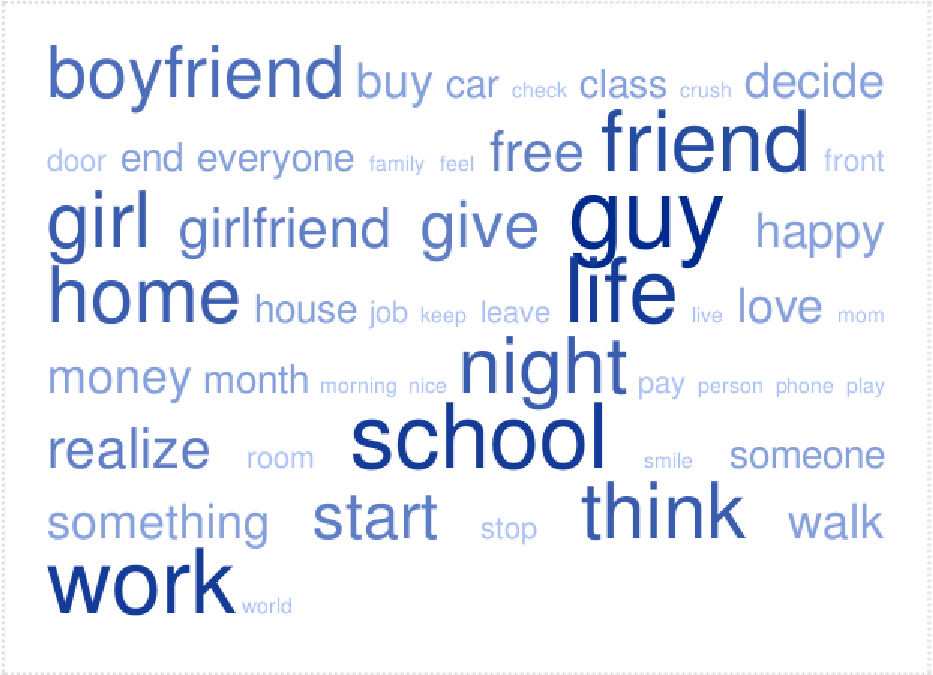
\includegraphics[width= 0.8 \columnwidth]{fig/pos_cloud}
\caption{Word cloud for documents with positive sentiment}
\label{fig:pos_cloud}
\end{figure}
%
\begin{figure}[!htp]
\centering
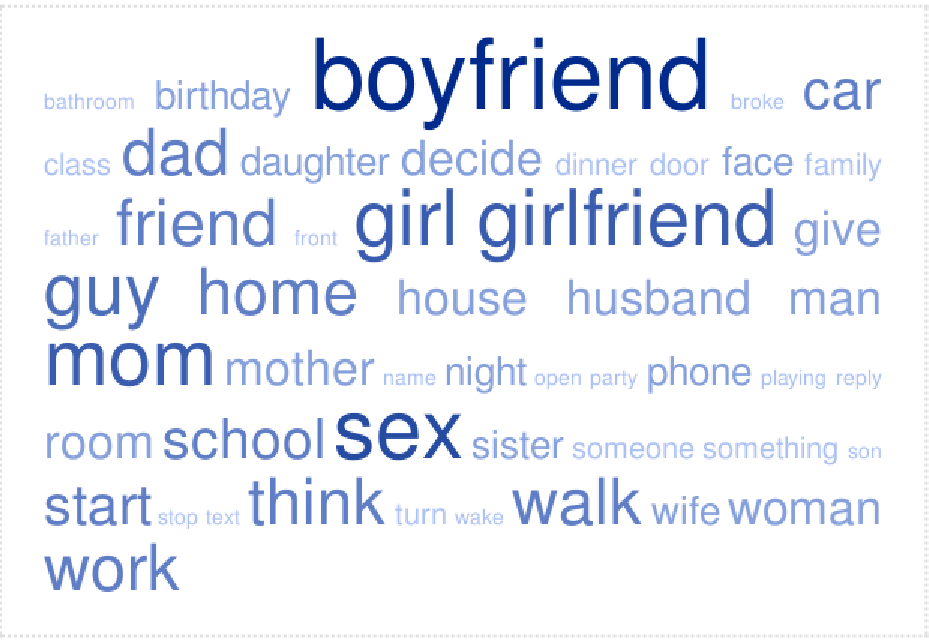
\includegraphics[width= 0.8 \columnwidth]{fig/neg_cloud}
\caption{Word cloud for documents with negative sentiment}
\label{fig:neg_cloud}
\end{figure}

\section{Feature representation}
\label{sec:features}

From the preceeding section, we obtain a set of short documents, let us cay them $D = \{d_1, d_2, \ldots, d_m\}$, with each document $i$ containing a possibly different set of words $w_{i} = \{w_{i,1}, w_{i, 2}, \ldots, w_{i, n_i} \}$. The purpose of this section is to select a good vocabulary of $n$ words, call it $W^*$, from the combined set of words, $W = \{w_1, \ldots, w_m\}$. Given such a set, we obtain a feature vector of length $n$ for every document $d_i$, say $x_i$.
$$
x_i[j] = \begin{cases}
	1 & \trm{ if } w_{i,j} \in W \\
	0 & \trm{ otherwise }
\end{cases}
$$
This results in a set of $n$-dimensional feature vectors $X = \{ x_1, x_2, \ldots, x_m \}$ with labels $Y = \{y_1, y_2, \ldots, y_m \}$. For some algorithms, we map the labels to binary classes, $C = \{c_1, c_2, \ldots, c_m \}$.
$$
c_i = \begin{cases}
	+ & \trm{ if } y_i > 0 \\
	- & \trm{ otherwise }
\end{cases}
$$

We employ four different feature representations:
\paragraph{Word Frequency}
\label{ssec:wf}
We can construct a word frequency map for every word $w \in W$ as,
$$
tf(w) = \sum_{i=1}^m [[ w \in w_i ]]
$$
The vocabulary $W^*$, is then set of words with $n$ highest frequencies.

\paragraph{Information Gain}
\label{ssec:ig}

\paragraph{Gain Ratio}
\label{ssec:gr}

\paragraph{TF-IDF}
\label{ssec:tfidf}
We also used an approach inspired from a popular method of constructing small vocabularies from a word corpus called ``term frequency-inverse document frequency''. The first term, i.e., term frequency is already computed in Sec.~\ref{ssec:wf}. Inverse document frequency is defined for a word $w \in W$ as
$$
idf(w) = \log \left[ \frac{m}{\abs{\{i: w \in w_i \}}} \right].
$$
The denominator here is the number of documents that a word $w$ appears in. Thus $idf$ penalises words which occur very frequently in documents. The vocabulary $W^*$ is constructed using the words with the highest value of the product $tf(w) * idf(w)$. In conventional TF-IDF formulations, each document has a large number of repeated words, e.g, research papers, which is not true in our case.

We note that this approach gives the best performance for a number of algorithms tested in this report.

\section{Preliminary results}
\label{sec:prelim}

This section uses the feature representation created in Sec.~\ref{sec:features} and shows an analysis of various algorithms and features on the data.
For the algorithms discussed in this section, we used a popular Python library for machine learning called $\tt scikit\_learn$~\cite{scikit-learn}. This library has very efficient and well documented implementations of algorithms which makes it possible to evaluate the performance with different values of parameters. We analyse the data using four different algorithms as described below:

\subsection{Support Vector Machine}
\label{ssec:svm}

\subsection{Principle Component Analysis}
\label{ssec:pca}


\subsection{Adaboost}
\label{ssec:adaboost}
%
Adaboost is a popular algorithm introduced by Freud and Schapire in~\cite{freund1999short}. The idea here is to fit a sequence of weak learners, e.g., one dimensional decision trees on slightly modified versions of the same data set. The predictions from all these weak learners (along with weights) are collected together to obtain the final classifier.

\subsection{Naive Bayes classifer}
\label{ssec:naive_bayes}
%
We are interested in calculating the probability of a label $+$ given all the words in a document, i.e., $\PP(+ \given w_1, \ldots, w_n)$. This can be written as,
\aeqs{
\PP(+ \given w_1, \ldots, w_n) &= \frac{\PP(+)\ \PP(w_1, \ldots, w_n \given + )}{\PP(w_1, \ldots, w_n)}\\
&\propto \PP(+, w_1, \ldots, w_n).
}
The numerator is a product of the prior probability of a class $+$ and the likelihood of generating $w_1, \ldots, w_n$ given $+$ to obtain the posterior on the left hand side. The Naive Bayes classifer works on the simple premise that the joint probability can be factorized as
$$
\PP(+, w_1, \ldots, w_n) = \PP(+) \prod_{i=1}^n \PP(w_i \given +)
$$
i.e., the probabiltiy of generating a class $+$ from individual words $w_i$ is independent of some other word $w_j$. A classifier can be obtained easily from this argument by as
$$
h(w_1, \ldots, w_n) = \arg \max_{c \in \{ +, - \} }\ \PP(c) \prod_{i=1}^n \PP(w_i \given c)
$$

In other words, it considers unigrams as independent of each other. Strictly speaking, this is not correct. As Fig.~\ref{fig:pos_cloud} and Fig.~\ref{fig:neg_cloud} show, there are quite a few common words in both data sets and a word like \emph{boyfriend} only shows a markedly different frequency in the two classes. However, for large amounts of data, this effect is less pronounced and we still obtain good classification.

\section{Latent topics}
\label{sec:latent}

The previous section demonstrated the performance of various classifers on the feature representations obtained from the data. This section builds upon the idea that words in a document are results of a few latent topics. In other words, rather than training a classifer to distinguish between words, we train it to distinguish between latent topics. The analysis in this section is inspired by~\cite{nikolov2012nonparametric}.

This idea has been pursued in literature in a number of different ways. Let us note a popular line of research that introduces supervised learning for topic models~\cite{blei2010supervised}. The idea here is to classify using 

Suppose that for the two classes, $+$ (documents that express positive sentiment) and $-$ (documents that express a negative sentiment), we have a set of latent topics. Let $p = \{ p_1, \ldots, p_m \}$ be the topics that result in words associated with $+$ and $q = \{ q_1, \ldots, q_n \}$ be the topics that result in words associated with $-$. Each sentiment $+$, $-$ is a noisy observation based upon these latent topics. However, we do not know what these topics are and hence we create a simple model for them.

Denote the words in a document by $s$. Let the probability of generating an observation $s$ from latent topics $p$ be,
$$
\PP(s\ \trm{generated from}\ p) \propto e^{-\gamma\ d(s, p)}
$$
where $d(s,p)$ is some positive definite function that metric and $\gamma$ is a tunable parameter. Note that we need $d(s,p)$ to be symmetric. In our work, we use the Hamming distance between two feature representations as the function $d(\cdot, \cdot)$. We make use of the set of observations, i.e., words in documents to classify a new document. Let $R_+$ be the set of all reference documents that are maked as $+$, $R_-$ is defined similarly. The probability of a new signal $s$ belonging to $+$ is then,

\aeqs{
\PP(+ \given s) &= \sum_{r \in R_+}\ \PP(s\ \trm{in}\ +, s\ \trm{shares a latent source with } r)\\
&= \sum_{r \in R_+} \sum_{j=1}^n \PP(s \trm{ generated by } p_j, r \trm{ generated by } p_j)\\
&\propto  \sum_{r \in R_+} \sum_{j=1}^n \exp(-\gamma[ d(s, p_j) + d(r, p_j)])\\
&\sim \sum_{r \in R_+} \exp \left( -\gamma \min_j [ d(s, p_j) + d(r, p_j)] \right)\\
&\sim \sum_{r \in R_+} \exp \left(-C\ \gamma d(s,r) \right).
}
The second last approximation is obtained as follows: We see that for a large $\gamma$, the summation $\sum_{j=1}^n$ is dominated by the term with the minimum exponent. On the other hand, the last approximation is obtained by noting that the minimum over all terms of the form $[ d(s, p_j) + d(r, p_j)]$ over all signals in $p$ is of the form $C d(s,r)$ for some $C > 0$ and is achieved at $p^* = (s+r)/2$. It is easy to see that this is a valid approximation when the latent source $p_{j^*}$ is close to the global minimizer $p^*$.

We can approximate $\PP(- \given s)$ similarly. The crux of this approach is that we cannot compare observations, i.e., words in documents to latent signals because we do not know them. Instead, we compare words to reference words in the traning data itself and obtain a simple rule for a discriminative classifier. Let $R(s) = \PP(+ \given s)/\PP(- \given s)$ and $\theta$ be a threshold. We classify the observation according to the function $f(s) = \trm{sign}(R(s) - \theta)$. It is clear that $\theta > 1$, we tuned $\theta$ and set its value to $1.25$ because we would like make fewer mistakes while classifying a tweet as $+$ (cite the walmart pregnancy example here).

\section{Conclusions}
\label{sec:conclusions}

\bibliography{writeup}
\bibliographystyle{unsrt}

\end{document}

